\documentclass[10pt, usenames, dvipsnames, xcolor=table]{beamer}
\usepackage[utf8]{inputenc}

\usefonttheme{structuresmallcapsserif}
\usetheme{Madrid}

\usepackage{esint}
\usepackage{tfm-miscelaneos}
\usepackage{sobolev} %https://ctan.math.illinois.edu/macros/latex/contrib/bosisio/sobolev.html
\usepackage{diffcoeff} %http://mirrors.ibiblio.org/CTAN/macros/latex/contrib/diffcoeff/diffcoeff.pdf

\usepackage{listings}
\usepackage{color}
\usepackage{xcolor}
\usepackage{graphicx}
\usepackage{subfigure}

\usepackage[T1]{fontenc}
\usepackage[british]{babel}
\usepackage{setspace}

\lstdefinestyle{Python}{
    language        = Python,
    basicstyle      = \ttfamily,
    keywordstyle    = \color{blue},
    keywordstyle    = [2] \color{teal}, % just to check that it works
    %stringstyle     = \color{green},
    commentstyle    = \color{red}\ttfamily
}

\graphicspath{ {./img/} }


%\usefonttheme[onlymath]{serif}
%\usepackage{amsfonts, amssymb, amsmath, amsthm}
%\usepackage{mathrsfs} %H de medida de Huasdorff
%\usepackage[inline]{enumitem}

%\usepackage{graphicx}
%\usepackage{animate}
%\usepackage{caption}
%\usepackage{xmpmulti}
%\usepackage{color}
%\usepackage{booktabs}
%\usecolortheme{whale}

 
%Information to be included in the title page:
\title[]{Birth-Death Process}
%\subtitle{\footnotesize Supervisors:  Frederic Nataf \& Taraneh Sayadi}
\author[Jose Manuel de Frutos]{\sc  Jose Manuel de Frutos}
\institute[]{\textbf {}}
%\titlegraphic{\includegraphics[width=2cm, height=1.2cm]{./img/logouam.pdf} \hspace{1cm} \includegraphics[width=2.2cm]{./img/logodpto.pdf}}

\date{\today}
  

\begin{document}


\frame{\titlepage}

\begin{frame}
  \frametitle{Index}
  \tableofcontents
\end{frame}

\section{Birth-Death Process Theory}
\begin{frame}
\frametitle{Birth-Death Process}

\begin{itemize}
\item Simple model of population dynamics called a birth-death processes. Population fluctuations (birth and death rates, $\beta_{birth}$ and $\beta_{death}$) depend only on the population size, $n$.

\item Let’s consider the following situation: protein synthesis. The rate at which the population increases depends only on the presence of the ingredients and is thus is fixed and a clearance rate (deaths) that is proportional to the total population, $n$.


\item Two possible events: births (or synthesis) and deaths (or decays).
\begin{align*}
\beta_{birth} = (constant)\\
\beta_{death}  = (k_0)*n
\end{align*}
\item $\beta_{birth}$  and $(k_0)$ are parameters of the model that would, in principle, be determined by experimental measurements. Both β rates have units of [events/time].
\end{itemize}
\end{frame}

\begin{frame}
\frametitle{Birth-Death Process}

\begin{itemize}
\item Deterministically, the population size $n$ can be described by the ordinary differential equation:
\begin{align*}
\frac{dn(t)}{dt} = b - b \cdot n(t)
\end{align*}
\item Solving this differential equation we get:
\begin{align*}
n(t) = c \cdot e^{-d\cdot t}+\beta/d
\end{align*}
Where $c=n(0)-\beta/d$.
\end{itemize}
\end{frame}

\begin{frame}
\frametitle{Extreme solutions}
Simplest cases of pure birth process and pure death process.
\begin{itemize}
\item \textbf{pure birth process}, the governing equation is: $n(t)=b\cdot t + n(0)$. So any numerical solution that we obtain has to follow a linear pattern of $\beta$ slope, for this case.
\item \textbf{pure death process}, the  governing equation is: $n(t)=e^{-d\cdot t}+n(0)-1$. In this case the decreasing exponential pattern has to be observed.
\item General equation, we obtain the asymptotic trend. With previous solution for the general problem: $n=\beta/d$. The concavity will depend on the value of $C$.
\end{itemize}
\end{frame}


\section{Stochastic Simulation Algorithm}
\begin{frame}
  \frametitle{Index}
  \tableofcontents[currentsection]
\end{frame}
\begin{frame}
\frametitle{Stochastic Simulation Algorithm}

\begin{itemize}

\item Two possible events that might occur and these might each happen at different rates: birth and death.

\begin{align*}
\frac{P_{death}}{P_{birth}+P_{death}}= \frac{d\cdot N}{\beta + d\cdot N}, \qquad \frac{P_{birth}}{P{death}+P_{birth}}= \frac{\beta}{\beta + d\cdot N}
\end{align*}

\item \textbf{Bernoulli Trial}. Event can either be a birth or a death, need to be able determine which event actually occured. We choose a random number between $(0,1)$ and see if it is less than $\frac{d\cdot N}{\beta + d\cdot N}$ or bigger. In each case we add or subtract an individual to the population (Monte-Carlo).

\item For simplicity and to avoid divisions, we take a random number between $(0,d\cdot N)$. And we check that it is less than or greater than $d\cdot N$.
\end{itemize}

\end{frame}


\begin{frame}
\begin{itemize}
\item Events in birth-death processes do not occur at regular time intervals; instead we can only say that the odds of an event occurring within any small time interval $\Delta t$ is equal to $a_{0} \Delta t$, where β is the mean rate of event occurrences. A sequence of random wait times is an example of what is called a ``Poisson Process."

\item Wait-times between sequential events follow an exponential distribution where the probability of the next event occurring after a duration $\tau$ (give-or-take $\Delta t$) is given by:

\begin{align*}
P(\tau) = a_{0} \cdot e^{-a_0 \cdot \tau}
\end{align*}

\item By \textbf{superposition property} we get that $\tau = - \frac{\log{r}}{\beta + d\cdot x}$. Where $r$ is a random number between $(0,1)$.
\end{itemize}
\end{frame}

\begin{frame}
\begin{figure}[h]
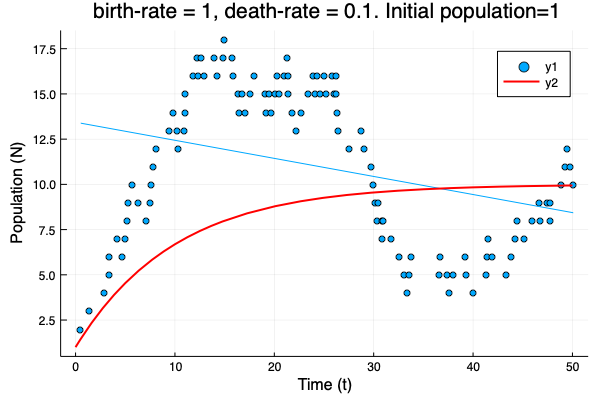
\includegraphics[width=4cm]{1_01_1}
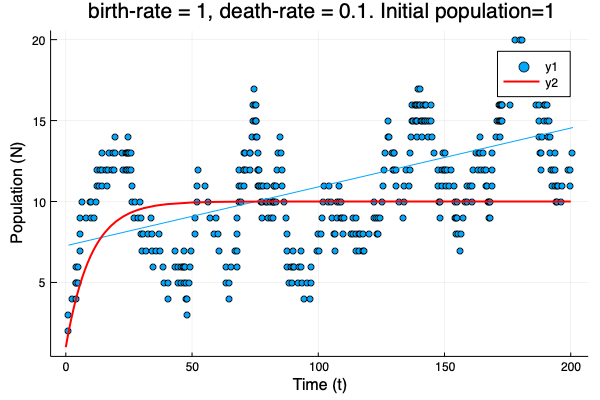
\includegraphics[width=4cm]{1_01_1_2}
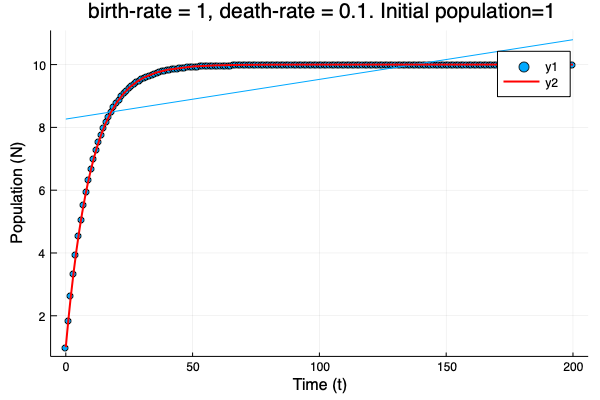
\includegraphics[width=4cm]{1_01_1_numerical}
%\caption{Some examples of simulation}
\end{figure}
\begin{figure}[h]
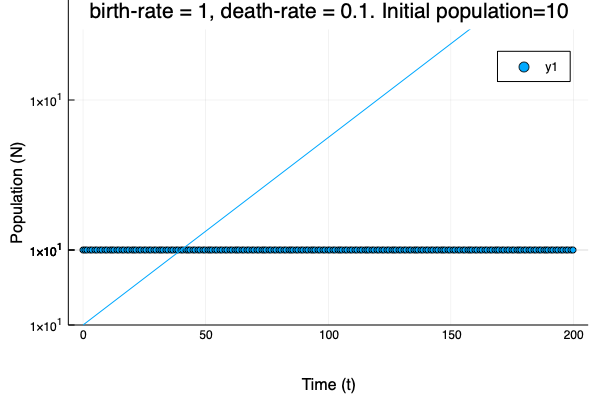
\includegraphics[width=4cm]{1_01_10}
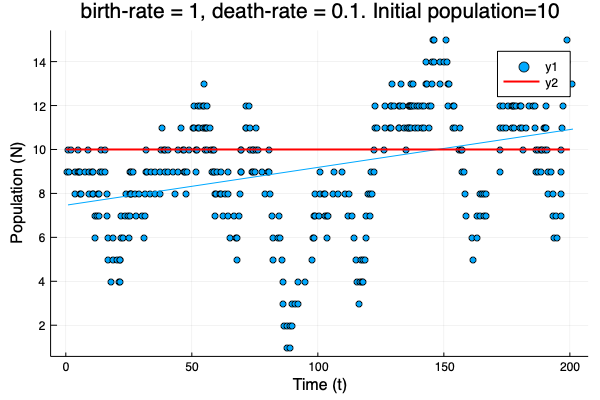
\includegraphics[width=4cm]{1_01_10_2}
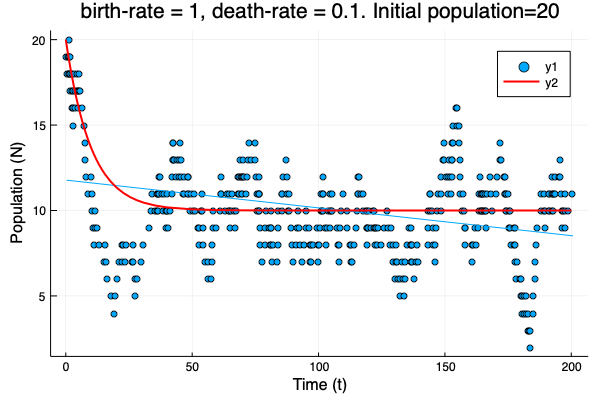
\includegraphics[width=4cm]{1_01_20}
\caption{Some examples of simulation}
\end{figure}
\end{frame}

\begin{frame}
\begin{figure}[h]
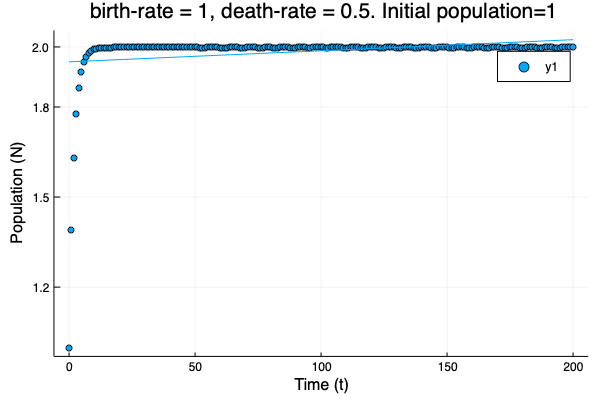
\includegraphics[width=4cm]{1_05_1}
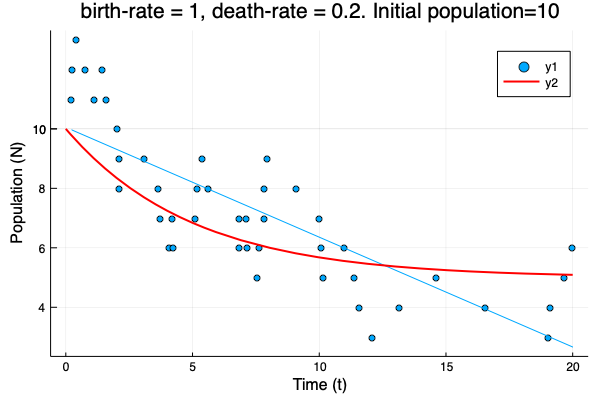
\includegraphics[width=4cm]{1_02_10}
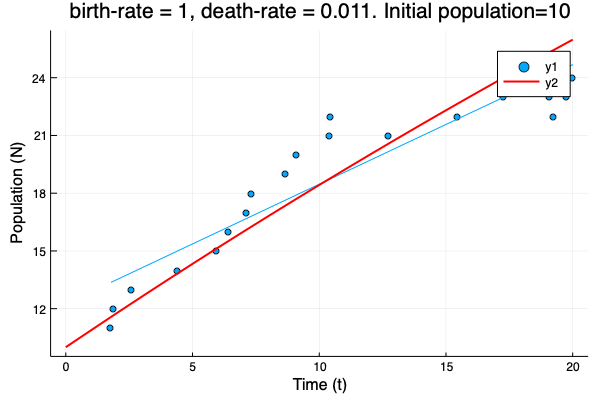
\includegraphics[width=4cm]{1_001_10}
%\caption{Some examples of simulation}
\end{figure}
\begin{figure}[h]
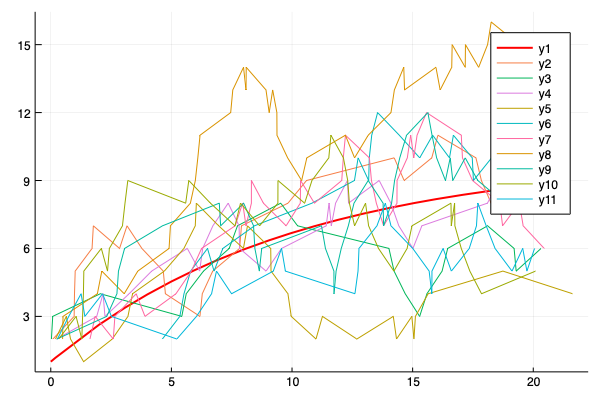
\includegraphics[width=6cm]{1_01_1_multiple}
%\caption{Some examples of simulation}
\end{figure}
\end{frame}

\section{Structure of BirthDeathProcess package}
\begin{frame}
  \frametitle{Index}
  \tableofcontents[currentsection]
\end{frame}
\begin{frame}
\frametitle{Structure of BirthDeathProcess package}
We have divided the package as follows:
\begin{itemize}
\item We have a file \textbf{Utils.jl} where we have the utility functions. Mainly we have the functionality to generate random numbers.
\item \textbf{DefaultParameters.jl} where we have the structure to define the parameters $\beta$ and $d$ of the model.
\item \textbf{Gillespie.jl} and \textbf{RungeKutta.jl} here we define the simulation algorithms.
\item We have separated the visualization and the obtaining of statistics in independent files. \textbf{Visualization.jl} and \textbf{Stats.jl}.
\item We expose the functions in the file \textbf{BirthDeathProcess.jl}.
\end{itemize}
Finally we have implemented tests and a documentation in html. These are located in the tests and doc folder.
\end{frame}

\begin{frame}
\frametitle{Github-ci workflow}
We have also implemented a github ci workflow. Find it ci.yml.
\begin{itemize}
\item Compiles the package for different versions of julia and in mac, windows and ubuntu environments.
\item Run the package tests. We have enabled a code coverage manager (codecov).
\item Generate the documentation. Created with Documenter.jl
\end{itemize}
\end{frame}


\nocite{*} 
\section{References}
\begin{frame}[allowframebreaks]
\frametitle{References}
\bibliographystyle{alpha}

\bibliography{ref_1}

\end{frame}




\end{document}
